%%%%%%%%%%%%%%%%%%%%%%%%%%%%%%%%%%%%%%%%%%%%%%%%%%%%%%%%%%%%%%%%%%%%%%%%%%%%%%%
\section[Section]{Classical cryptography}
\part{Classical cryptography}

%%%%%%%%%%%%%%%%%%%%%%%%%%%%%%%%%%%%%%%%%%%%%%%%%%%%%%%%%%%%%%%%%%%%%%%%%%%%%%%
\begin{frame}{Caesar cipher}

\centering

\smallskip

Encrypt: \textcolor{red}{right shift} each letter of 3 positions

\smallskip

Decrypt: \textcolor{red}{left shift} each letter of 3 positions

\medskip

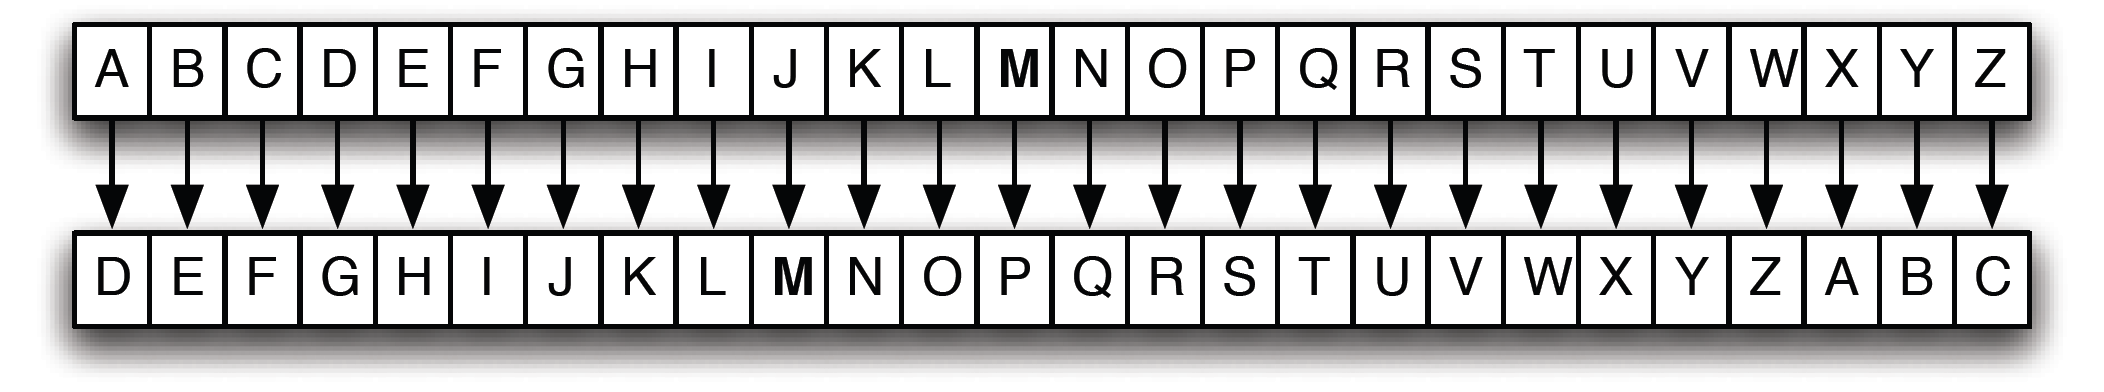
\includegraphics[width=10cm]{img/caesar-shift.png}

\medskip

General cipher: shift letter of $K$ positions

\smallskip

Attack: \textcolor{red}{bruteforce} all the possible $K$ (only $25$ values...)

\end{frame}

%%%%%%%%%%%%%%%%%%%%%%%%%%%%%%%%%%%%%%%%%%%%%%%%%%%%%%%%%%%%%%%%%%%%%%%%%%%%%%%
\begin{frame}{ROT\{13, 47\}}

\centering

\medskip

ROT13: Caesar cipher with $K = 13$ on alphabetic dictionary

ROT47: Caesar cipher with $K = 47$ on printable ASCII chars (33 - 126).

\medskip

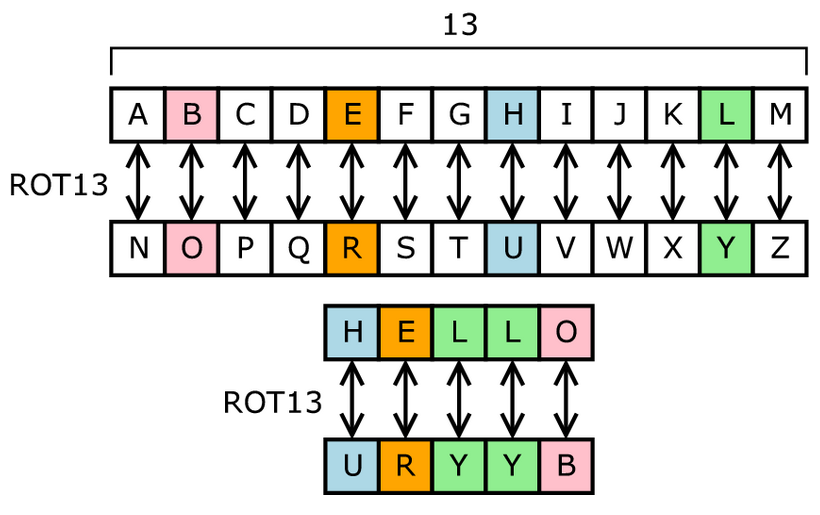
\includegraphics[width=8cm]{img/ROT13.png}

\medskip

Why $K = 13$ (or $K = 47$)? Because \textcolor{red}{Encrypt = Decrypt}

\end{frame}

%%%%%%%%%%%%%%%%%%%%%%%%%%%%%%%%%%%%%%%%%%%%%%%%%%%%%%%%%%%%%%%%%%%%%%%%%%%%%%%
\begin{frame}{Classical ciphers}

\textbf{Substitution ciphers}

\phantom{pad}- Monoalphabetic ciphers: \textcolor{red}{$C_{new} = P[C_{old}]$} (Where $P$ is a dictionary permutation)

\smallskip

\phantom{pad}(ROT-K is a monoalphabetic cipher with $P$ is a cyclic rotation)

\smallskip

\phantom{pad}- Polialphabetic ciphers: \textcolor{red}{multiple substitution} alphabets 

\phantom{pad}(more than one dictionary permutation)

\smallskip

\textbf{Transposition ciphers}

\phantom{pad}Encryption systems where the \textcolor{red}{positions} held by units of plaintext 

\phantom{pad}(characters or groups of characters) \textcolor{red}{are shifted} according to a regular system.

\smallskip

E.g. We want to encrypt the message \textit{WE ARE DISCOVERED. FLEE AT ONCE} using the \textbf{route cipher}:

Grid: 

\centerline{\texttt{W R I O R F E O E}}
\centerline{\texttt{E E S V E L A N J}}
\centerline{\texttt{A D C E D E T C X}}

Cipher text: \textit{EJXCTEDECDAEWRIORFEONALEVSE}

\end{frame}
%%%%%%%%%%%%%%%%%%%%%%%%%%%%%%%%%%%%%%%%%%%%%%%%%%%%%%%%%%%%%%%%%%%%%%%%%%%%%%%
\begin{frame}{Polialphabetic substituion cipher: Vigenère}
  
The problem with monoalphabetic ciphers is that each character of the alphabet is replaced with always the same character in the ciphertext.

\smallskip

What can we do to solve this weakness? \textcolor{red}{Stack more ciphers}!

The Vigenère cipher is basically a \textbf{sequence of Caesar ciphers with different shifts}.

\smallskip

  \begin{columns}
  \begin{column}{0.4\textwidth}

    \centerline{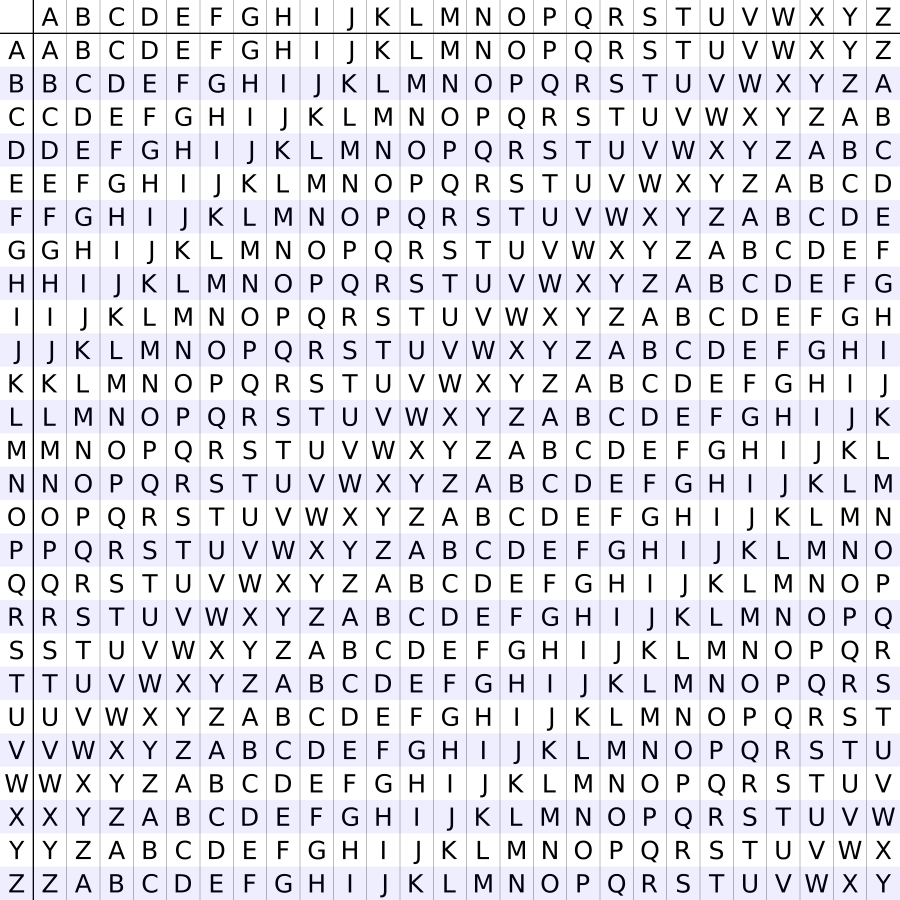
\includegraphics[width=4cm]{img/VigenereTable.png}}

    This table is called \textcolor{red}{Vigenère table}.
    
    It contains all the Caesar ciphers. 

  \end{column}
  \begin{column}{0.6\textwidth}


    Encryption is performed character-by-character by accessing the cell of the table within the row corresponding to the current key letter and column to the plaintext letter.

    Decryption works in the same way of the encryption but we use a transposed Vigenère table.

    This simple technique earned the name of \textcolor{red}{the indecipherable cipher}, and resisted attacks for over 3 centuries (1553-1863)!

  \end{column}
  \end{columns}



\end{frame}
%%%%%%%%%%%%%%%%%%%%%%%%%%%%%%%%%%%%%%%%%%%%%%%%%%%%%%%%%%%%%%%%%%%%%%%%%%%%%%%
\begin{frame}{Vigenère cipher: an example}
  
  We want to encrypt the message \texttt{THIS IS AN EXAMPLE} with the key \texttt{SECRET}

  \medskip
  
  First of all, we repeat the key until it has the same length of the plaintext: \\

  \medskip
  
  $m =$ \texttt{THISISANEXAMPLE}\\
  $k =$ \texttt{SECRETSECRETSEC}\\

  \medskip
  
  In our example, the first letter of the plaintext is $T$ and the first of the key is $S$, so we access the row $S$ and column $T$, which yields $L$. 
  
  And so on until the end of the message:\\

  \medskip
  
  $c =$ \texttt{LLKJMLSRGOEFHPG}

\end{frame}
%%%%%%%%%%%%%%%%%%%%%%%%%%%%%%%%%%%%%%%%%%%%%%%%%%%%%%%%%%%%%%%%%%%%%%%%%%%%%%%
\begin{frame}{Transposition cipher: an example}

The plaintext is written in a rectangular grid and then the columns are reshuffled, the encryption key is the \textcolor{red}{column permutation}

\medskip

$m =$ \texttt{THIS IS AN EXAMPLE}\\
$k =$ \texttt{\{4, 2, 1, 3\}}

\medskip

\centerline{\texttt{T H I S  \phantom{-------------------->} S H T I}}
\centerline{\texttt{I S A N  \phantom{---}Reorder columns\phantom{---} N S I A}}
\centerline{\texttt{E X A M  \phantom{---}-------------->\phantom{---} M X E A}}
\centerline{\texttt{P L E =  \phantom{-------------------->} = L P E}}

\medskip

$c =$ \texttt{SHTINSIAMXEA=LPE}

\medskip

To recover the original message, just write the ciphertext in a grid again and apply the inverse permutation of columns

\end{frame}
%%%%%%%%%%%%%%%%%%%%%%%%%%%%%%%%%%%%%%%%%%%%%%%%%%%%%%%%%%%%%%%%%%%%%%%%%%%%%%%
\begin{frame}{dcode.fr}

\centering

\href{https://www.dcode.fr/tools-list}{https://www.dcode.fr/tools-list}

\medskip

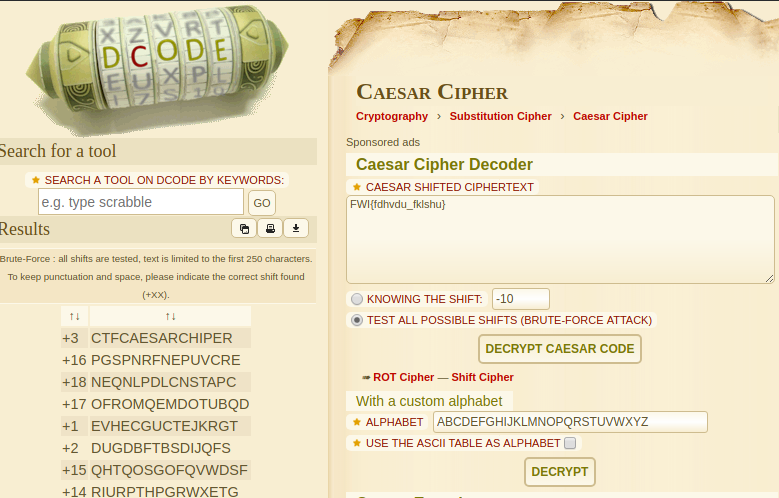
\includegraphics[width=8cm]{img/dcode.png}

\medskip

\textcolor{red}{Almost} all possible classic ciphers (old and new), encoder/decoder, ...

\end{frame}
%%%%%%%%%%%%%%%%%%%%%%%%%%%%%%%%%%%%%%%%%%%%%%%%%%%%%%%%%%%%%%%%%%%%%%%%%%%%%%%
\begin{frame}{Cryptanalysis}

Often the vulnerability is not in the algorithm but in \textcolor{red}{its application}...

\begin{itemize}
  \item Bad use of the key (too short, reused, bad generated, ...)
  \item Messages use a poorly distributed dictionary
  \item We know the message format (e.g.: \textsc{flag\{\ldots\}})
\end{itemize}

\medskip

In particular we talk about \textcolor{red}{statistical cryptanalysis} when we force the cipher not from algorithmic point of view but from statistical one

\medskip

For example in english the character E has a frequency of 12.02\% while Z only 0.07\%

\medskip

Useful tool (for substitution ciphers): \href{https://quipqiup.com}{https://quipqiup.com}

\medskip

\centering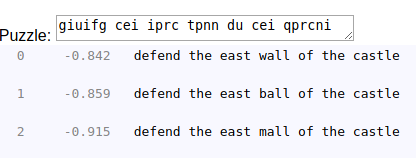
\includegraphics[width=5cm]{img/quipqiup.png}
  
\end{frame}
%%%%%%%%%%%%%%%%%%%%%%%%%%%%%%%%%%%%%%%%%%%%%%%%%%%%%%%%%%%%%%%%%%%%%%%%%%%%%%%

\begin{frame}{Attack models}

Classification of cryptographic attacks:

\medskip

\begin{itemize}
  \item \textcolor{red}{Ciphertext-only} attack: access only to the ciphertext, and has no access to the plaintext
  \medskip
  \item \textcolor{red}{Known-plaintext} attack: access to at least a limited number of pairs of plaintext and the corresponding enciphered text
  \medskip
  \item \textcolor{red}{Chosen plaintext} attack: able to choose a number of plaintexts to be enciphered and have access to the resulting ciphertext (encrypt oracle)
  \medskip
  \item \textcolor{red}{Chosen ciphertext} attack: able to choose arbitrary ciphertext and have access to plaintext decrypted from it (decrypt oracle) 
  \medskip
  \item \textcolor{red}{Side-channel} attack: use of other informations to break the cipher (time, sound, power, error, ...).
\end{itemize}
  
\end{frame}
%%%%%%%%%%%%%%%%%%%%%%%%%%%%%%%%%%%%%%%%%%%%%%%%%%%%%%%%%%%%%%%%%%%%%%%%%%%%%%%
